% This file contains text to create bios for EnICS members and close collaborators

%<*AdamTeman>
\begin{IEEEbiography}    [{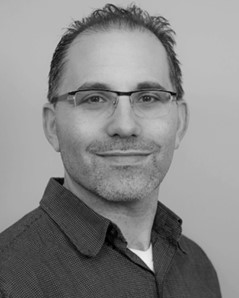
\includegraphics[width=1in,height=1.25in,clip,keepaspectratio]{./Bios/adam_teman.jpg}}]
    {Adam Teman} (Member, IEEE) received the Ph.D. degree in electrical and computer engineering from Ben-Gurion University (BGU), Be’er Sheva, in 2014. He worked as a Design Engineer at Marvell Semiconductors, from 2006 to 2007. From 2014 to 2015, he was a Postdoctoral Researcher at the École Polytechnique Fédérale de Lausanne (EPFL), Switzerland, under a Swiss Government Excellence Scholarship. Since 2015, he has been with Bar-Ilan University, where he is an Associate Professor and the Co-Director of the Emerging Nanoscaled Integrated Circuits and Systems (EnICS) Laboratories. In 2021, he co-founded RAAAM Memory Technologies, where he is head of Product Development. He has authored over 115 scientific articles and holds 11 patents. His research interests include embedded memories, energy-efficient circuit design, hardware for artificial intelligence, open source processor platforms and accelerators, and methodologies for physical implementation. In 2020, he was awarded the Krill Prize for outstanding young researchers. 
\end{IEEEbiography}
%</AdamTeman>

%<*LeonidYavits>
\begin{IEEEbiography}[{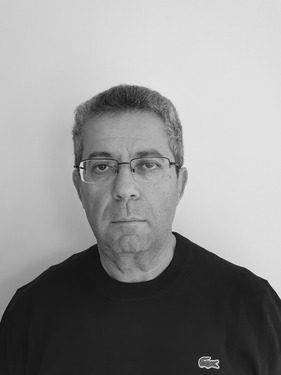
\includegraphics[angle=0,width=1in,height=1.25in,clip,keepaspectratio]{./Bios/leonid_yavits.jpg}}]{Leonid Yavits} 
    is with the Faculty of Engineering, Bar-Ilan University, Israel. He received his MSc and PhD degrees in electrical engineering from Technion, Israel. Leonid is a serial entrepreneur who was involved in co-founding and successful management (from a concept to M\&A) of several start-ups in the field of ASICs. His research interests include bioinformatics, domain specific accelerators, and processing in memory.
\end{IEEEbiography}
%</LeonidYavits>

%<*AlexFish>
\begin{IEEEbiography}    [{\includegraphics[width=1in,height=1.25in,clip,keepaspectratio]{./Bios/alex_fish.jpg}}]
    {Alex Fish} (Member, IEEE) . 
\end{IEEEbiography}
%</AlexFish>

%<*YossieShor>
\begin{IEEEbiography}    [{\includegraphics[width=1in,height=1.25in,clip,keepaspectratio]{./Bios/yossie_shor.jpg}}]
    {Yossie Shor} (Senior Member, IEEE) . 
\end{IEEEbiography}
%</YossieShor>

%<*ItamarLevy>
\begin{IEEEbiography}    [{\includegraphics[width=1in,height=1.25in,clip,keepaspectratio]{./Bios/itamar_levy.jpg}}]
    {Itamar Levy} (Member, IEEE) . 
\end{IEEEbiography}
%</ItamarLevy>

%<*OsnatKeren>
\begin{IEEEbiography}    [{\includegraphics[width=1in,height=1.25in,clip,keepaspectratio]{./Bios/osnat_keren.jpg}}]
    {Osnat Keren} (Member, IEEE) . 
\end{IEEEbiography}
%</OsnatKeren>


%%%%%%%%%%%%%%%%%%%%%%%%%%%%%%%%%%%%%%%%%%%%%%%%%%%%
%%%                  UNICAL                      %%%
%%%%%%%%%%%%%%%%%%%%%%%%%%%%%%%%%%%%%%%%%%%%%%%%%%%%
%<*EstebanGarzon>
\begin{IEEEbiography}[{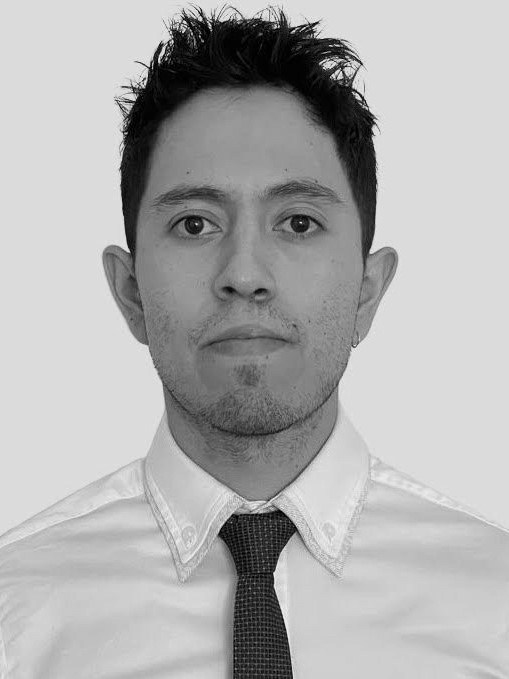
\includegraphics[width=1in,height=1.25in,clip,keepaspectratio]{./Bios/esteban_garzon.jpg}}]{Esteban~Garzón}
    (Member, IEEE) received the Ph.D. degree in electronics engineering from the University of Calabria (UNICAL), Italy, in 2022. He is currently a Postdoctoral Researcher at the Department of Computer Engineering, Modeling, Electronics and Systems Engineering, UNICAL. He has coauthored more than 30 scientific papers in international journals and conferences, and has participated in several IC tapeouts. His research interests include domain-specific hardware accelerators, and electronics/spintronics, cryogenic memories, and standard and emerging technologies for logic, memory, and low-power applications. 
\end{IEEEbiography}
%</EstebanGarzon>

%<*MarcoLanuzza>
\begin{IEEEbiography}[{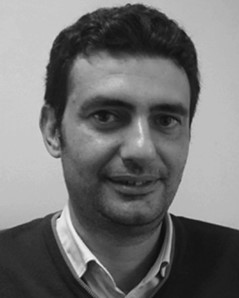
\includegraphics[width=1in,height=1.25in,clip,keepaspectratio]{./Bios/marco_lanuzza.jpg}}]{Marco Lanuzza}
    (Senior Member, IEEE) received the Ph.D. degree in electronic engineering from the Mediterranea University of Reggio Calabria, Reggio Calabria, Italy, in 2005. Since 2006, he has been with the University of Calabria, Rende, Italy, where he is currently an Associate Professor. He has authored over 120 publications in international journals and conference proceedings. His recent research interests include the design of ultralow voltage circuits and systems, the development of efficient models and methodologies for leakage- and variability-aware designs, and the design of digital and analog circuits in emerging technologies. Prof. M. Lanuzza is an Associate Editor of Integration, the VLSI Journal.
\end{IEEEbiography}
%</MarcoLanuzza>


